\chapter{Design and Translation}
\label{design_translation}
In this chapter, the extension of mbeddr for parallel programming, called ParallelMbeddr, is introduced. To this end, the new language features for C are explained, each in terms of their design and the translation to plain mbeddr C code.\footnote{For the sake of legibility, the syntax of the generated mbeddr code is depicted in a simplified manner where deemed necessary.} In order to illustrate the presented features, a running example is incrementally built. Further examples are depicted whenever the running example does not provide the right structure to clarify a feature. At the end of this chapter, the measures implemented to make the extension sufficiently thread-safe\footnote{Data-races should be prevented as well as possible. However, the user always has the opportunity to introduce data races if his requested synchronizations for the modifications of data, which are used by multiple units of execution, do not correctly take into account the data dependencies of variables.} are explained.

\subsubsection{Notation}
In the following sections, the concepts of the language of mbeddr are iteratively extended with new elements. For this purpose, based on the notation presented by Pierce \cite{TypesAndProgrammingLanguages}, the syntax of new concepts is described by notations like the following:
\begin{equation}
e ::= ...| e'
\end{equation}
This exemplary line extends the set of expressions of mbeddr by the expression \CODE{e'} which may contain arbitrary meta-variables like \CODE{e}. In order to fit into the type system of mbeddr, these concepts are equipped with \textit{type inference} rules, each of which, given a list of premises, derives the type of some concept in the conclusion:
\begin{equation}
\inference*[NewConcept]{\mathit{premise_1}, ..., \mathit{premise_n}}{\qquad\quad e' |- t' \qquad\quad} 
\end{equation}
The premises of the concepts are kept minimal but not exhaustive, which means that complex premises are given as informal explanations and are mostly explained in section \ref{safetyMeasures}. This way, the type inference rules are kept comprehensible and the explanations for the safety measures of ParallelMbeddr are kept closely together. Additionally, this separation resembles MPS' separation of type inference rules and non-typesystem rules.

The translation of a new concept in ParallelMbeddr to a base concept of mbeddr will be shown informally by listing the resulting code that is generated by the IDE after it was given some input code. To this end, if not expressed in the text, the symbol $\Longrightarrow$ will denote the translation of code $c_1$ to some other code $c_2$ in $c_1 \Longrightarrow c_2$. The translation of basic code will often entail the generation of additional code somewhere else in the program as a side effect, e.g. the translation of an expression to a function call may force the generator of mbeddr to generate the declaration of the called function first. These side effects will also be demonstrated by listings of the generated code.
\section{Tasks}
The basic parallelization element is a \textit{task}. It denotes a parallel unit of execution and, as the name suggests, aims at task parallelism. As the implementation of the underlying parallelization technique might change in the future it is reasonable to abstract the terminology from it. The most basic task which always exists executes the code of the entry (main) function of the program. A task can also be regarded as a closure of the expression that shall be run in parallel. The reader should distinguish this `execution template' from the actual running instance of a task. The latter will further on be addressed as a \textit{running task}.
\subsection{Design}
\label{tasksDesign}
The syntax \texttt{e} of expressions in mbeddr is extended by
\begin{equation}
e ::= ...|\;\mathit{|e|}
\end{equation}

When executed, a task term yields a handle to a parallel unit of execution. This way, the initialization of the task and the actual execution are decoupled and can happen independently. When a task is run the embraced expression is executed and its value is returned. If the type of the expression is \textit{void} then no value will be returned. The type of a task reflects its return value:

\begin{equation}
t ::= ... |\;\mathit{Task{<}t{>}}
\end{equation}

Due to implementation reasons (see \ref{futuresTranslation} for details), the embraced return type of a task must be either \textit{void} or a pointer to the type of the embraced expression:

\begin{equation}
\inference*[VoidTask]{e |- \mathit{void}}{|e| |- \mathit{Task{<}void{>}}} 
\qquad\qquad
\inference*[NonVoidTask]{e |- t & t \neq \mathit{void}}{|e| |- \mathit{Task{<}void{\text{*}}{>}}}
\end{equation}

When a task is not used anymore to produce running instances of itself, it should be cleared in order to free the memory that it implicitly occupies in the heap:

\begin{equation}
e ::= ...|\;e.\mathit{clear}
\end{equation}
\begin{equation}
\inference*[Clear]{|e| |- \mathit{Task{<}t{>}}}{e.\mathit{clear |-} \mathit{void}} 
\end{equation}

If a task (template) is copied by the pass-by-value semantics of C, the copied task will share the heap-managed data, i.e. the reference environment of its free variables, with the original task. Therefore, a task needs to be cleared only once in order to avoid memory leaks. It has to be kept in mind that a running instance of a task will not be affected by the clearance of its task template. The clearance of a task is only necessary if the task is stored somewhere. Thus, a task that is directly run via \CODE{|e|.run} does need not to be cleared, which makes such expressions memory-safe.

\subsection{Translation}
\label{tasksTranslation}
The \textit{POSIX Threads} standard and library (pthreads) was chosen as a means to realize concurrency in the translated code. It supports all necessary parallelization features and provides a more direct control of the generated code when compared to frameworks like \textit{OpenMP}.\footnote{http://openmp.org/} Every task in ParallelMbeddr is represented by a thread as provided by the POSIX threads standard, a so-called \textit{pthread}.\footnote{In the following sections, \textit{pthreads} will denote both the library and multiple thread instances of the library. The context should always implicitly clarify which one is currently meant.} As the thread initialization function of pthreads takes a function pointer of type \CODE{void* -> void*}, the computation of the translated task is represented by an according function:

\begin{ccode}{caption=Generated function of a task}
void* parFun_X(void* voidArgs) {...}
\end{ccode}

The \CODE{X} in the name indicates that for every task a unique adaptee of this function with the prefix \CODE{parFun\_} and some unique suffix chosen by the framework is generated.\footnote{In the following explanations, \CODE{X} will always denote some arbitrary suffix. It has to be kept in mind, though, that these suffixes do not necessarily coincide with each other for different kinds of components.} As the function signature indicates, a pthread and therefore a task which is to be run can be parameterized with values and can return a value which will be explained in the following paragraphs.

If a task contains any references to local variables or function arguments, they need to be bound to capture the variable states at the time of the task initiliazation. Such states are represented by an `argument' struct:

\begin{ccode}{caption=Struct for a task expression with references \CODE{v\_1} to \CODE{v\_n}}
struct Args_X {
  t_1 v_1;
  ...
  t_n v_n;
}
\end{ccode}

where in the task expression every \CODE{v\_i} represents an equally named reference to a variable or argument of type \CODE{t\_i}. The generated function \CODE{parFun\_X} is then given an instance of \CODE{Args\_X}, which it uses to bind the references of the task expression to. The full function definition of a task \CODE{e} of type \CODE{Task<t*>} is, thus:

\begin{ccode}{caption=Structure of the generated function of a task}
void* parFun_X(void* voidArgs) {
  t* result = malloc(sizeof(t));
  Args_X* args = (Args_X*) voidArgs;
  *result = e';
  free(voidArgs);
  return result;
}
\end{ccode}

where \CODE{e'} is the expression obtained when every local variable reference and function argument reference \CODE{r} in \CODE{e} is substituted by a reference to an equally named and typed field in \CODE{args}:
\begin{equation}
r\;/\;\mathit{args}\text{-->}r
\end{equation}
If the embraced expression of a task does not contain any reference of this kind (e.g. only references to global variables) the argument related lines 3 and 5 are omitted as is clearly the -- otherwise empty -- declaration of \CODE{struct Args\_X}. In this case \CODE{e'} equals \CODE{e} except for other reductions of \CODE{e} that might occur in the translation process of mbeddr.

The generated function of a task of type \CODE{Task<void>} omits the result-related statements:

\begin{ccode}{caption=Structure of the generated function of a \CODE{void} task, label=lst:parFunDeclaration}
void* parFun_X(void* voidArgs) {
  t* result = malloc(sizeof(t));
  Args_X* args = (Args_X*) voidArgs;
  e';
  free(voidArgs);
}
\end{ccode}

Again, any argument-related code is generated as needed.

The aforementioned handle that a task yields is represented by an instance of a corresponding struct which captures both the initialization state and the computation of the embraced expression.\footnote{\CODE{(void*) => (void*) fun} is mbeddr syntax for the not easily edible function pointer \CODE{void *(*fun) (void *)} in standard C99.} The \textit{void} pointer of the arguments \CODE{voidArgs} does not keep the arguments' type information and with it their byte size. Therefore, an additional field \CODE{argsSize} is needed in order to be able to create copies of the arguments later on (see \ref{futuresTranslation} for details).
\begin{ccode}{caption=Generic struct generated for tasks}
exported struct Task {
  void* args;
  (void*) => (void*) fun;
  size_t argsSize;
}
\end{ccode}

As opposed to the unique definitions of other elements that need to be defined for every occurrence of a task (the ones with the \CODE{X} suffixes), \CODE{struct Task} is generic and is reused for every task. Generic declarations are kept in fixed, separately generated modules (in which code is organized in mbeddr) and are imported into the user-defined modules.
With these components in mind, the actual translation of a task expression \CODE{|.|} that contains references \CODE{v\_1} to \CODE{v\_n}, which need to be bound, becomes an mbeddr block expression:\footnote{A block expression contains a list of statements of which the mandatory yield statement returns the result value.}

\begin{minipage}{1\textwidth}
\begin{center}
\begin{minipage}{0.35\textwidth}
\begin{ccode}{}
{
  Args_X* args_X = 
    malloc(sizeof(Args_X));
  args_X->v_1 = v_1;
  ...
  args_X->v_n = v_n;
  yield (Task){ args_X, parFun_X, 
                sizeof(Args_X) };
}
\end{ccode}
\end{minipage}
\begin{minipage}{0.1\textwidth}
\quad$\Longrightarrow$\qquad
\end{minipage}
\begin{minipage}{0.5\textwidth}
\begin{ccode}{}
taskInit(v_1, ..., v_n)
\end{ccode}
with function declaration
\begin{ccode}{}
inline Args_X taskInit(t_1 v_1, ..., t_n v_n) {
  Args_X* args_X = malloc(sizeof(Args_X));
  args_X->v_1 = v_1;
  ...
  args_X->v_n = v_n;
  return (Task){ args_X, parFun_X, 
                 sizeof(Args_X) };
}
\end{ccode}
\end{minipage}
\end{center}
\captionof{lstlisting}{Reduction of a task expression to a block expression and further on to a function call}
\label{lst:taskReduction}
\end{minipage}
\vspace*{4mm}

The expression of the \CODE{yield} statement is a C \textit{compound literal}, which on evaluation creates an instance of the aforementioned \CODE{struct Task}. The block expression is then further reduced by mbeddr to a call of a newly generated inline function.\footnote{Whereas in C for a struct type \CODE{T}, a typedef has to be manually defined by the programmer, this definition is done implicitly in mbeddr, in order to reference this type directly with \CODE{T} instead of \CODE{struct T}.} Without any references to bind, a task is reduced to the compound literal:

\begin{ccode}{caption=Reduction of a task without references to bind}
(Task_X){ null, parFun_X, 0 }
\end{ccode}

The reduction of a task is accomplished differently if the task is immediately run via \CODE{|e|.run}. Section \ref{futuresTranslation} will show how this is done. By the definition of \CODE{Args\_X} in listing \ref{lst:taskReduction}, it becomes clear that, due to the call of \CODE{malloc} in line 3, the arguments of a task -- its environment -- are stored in the heap before execution.\footnote{This memory allocation in the heap should not be mixed up with the one in line 2 of listing \ref{lst:parFunDeclaration} which will be explained later on.} This approach was chosen mainly in order to simplify the generation of the resulting code. In consequence, the arguments of a task (template) have to be deleted by the programmer by hand with \CODE{e.clear}. However, one advantage of the chosen implementation is that a task may be passed by value, e.g. when using a builder function to create tasks, without the possible need to copy multiple arguments. Instead just the pointer to the heap-managed data is copied. The results of tasks also reside in the heap, for reasons which are explained later, and must therefore be manually deleted, as well (with the standard C function \CODE{free}). For this reason, it becomes apparent that the return type of a task must either be a void type or a pointer type, as was mentioned in the design section.   

In the translated code, the clearance \CODE{e.clear} of a task becomes a call of the \CODE{free} function of C, parameterized with the arguments of the translated task \CODE{e'}:
\begin{ccode}{caption=Reduction of a task clearance expression}
free(e'.args)
\end{ccode}

\subsection{Example Code}
\label{taskExample}
The running example concerns itself with the calculation of $\pi$, based on the definition given in the concurrent-pi example for the programming language \textit{Go}.\footnote{https://github.com/foamdino/learning-go/blob/master/concurrent-pi/concurrent-pi.go} $\pi$ is approximated by the summation of a certain number \textit{n} of terms where \textit{n} determines the deviation of the result from the actual value of $\pi$, i.e. the result's precision: 
\begin{equation}\label{eq:pi}
{\pi}_{\mathrm{approx}} = \sum\limits_{i=0}^{n}4*{-1^i \over 2i+1}
\end{equation}
In the first scenario, the amount of work is distributed among a certain number of tasks, each of which calculates the contribution of summands for a range of indices \textit{i}. The calculation of such a partial sum for a range $[\mathrm{start}, \mathrm{end}[$ (block) of indices is done by the functions:
\begin{ccode}{caption=Calculation of $\pi$ via equation \ref{eq:pi}}
long double calcPiBlock(uint32 start, uint32 end) { 
  long double partialSum = 0; 
  for (uint32 i = start; i < end; ++i) { partialSum += calcPiItem(i); }
  return partialSum; 
}
 
long double calcPiItem(uint32 index) { 
  return 4.0 * (pow (-1.0, index) / (2.0 * index + 1.0)); 
}
\end{ccode}
The work can be distributed among e.g. 4 tasks, where each task calculates a partial sum for an equally long block, which is given by:
\begin{ccode}{}
#constant BLOCKSIZE = 300000000;
#constant BLOCKCOUNT = 4; 
#constant THRESHOLD = BLOCKSIZE * BLOCKCOUNT;
\end{ccode}
These values are then used to initialize an array of tasks:
\begin{ccode}{caption=Main function of parallel $\pi$ calculation}
int32 main(int32 argc, string[] argv) {
  ...
  Task<long double*>[BLOCKCOUNT] calculators;
  for (i ++ in [0..BLOCKCOUNT[) { 
    uint32 start = i * BLOCKSIZE; 
    uint32 end = start + BLOCKSIZE; 
    calculators[i] = |calcPiBlock(start, end)|; 
  } ...
}
\end{ccode}
The final summation of the calculated blocks will be shown after the presentation of futures in section \ref{futuresExample}. The code is translated\footnote{For legibility reasons, the code shown in the following listing and any other mbeddr code presented is a simplified version of the intermediate code that mbeddr actually generates. The performed changes are restricted to renaming and negligible syntax changes.} to the building blocks that were introduced in \ref{tasksTranslation}:
\begin{ccode}{caption=Reduced code of parallel $\pi$ calculation}
int32 main(int32 argc, string[] argv) {
...
  Task[BLOCKCOUNT] calculators;
  for (int8 __i = 0; __i < BLOCKCOUNT; __i++) { 
    uint32 start = __i * BLOCKSIZE; 
    uint32 end = start + BLOCKSIZE; 
    calculators[__i] = taskInit_0(start, end); 
  }
...
}

struct Args_0 { 
  uint32 start; 
  uint32 end; 
};

inline Task taskInit_0(uint32 start, uint32 end) { 
  Args_0* args_0 = malloc(sizeof(Args_0)); 
  Args_0->start = start; 
  Args_0->end = end; 
  return (Task){ args_0 , :parFun_0 , sizeof (Args_0)}; 
}

void* parFun_0(void* voidArgs) { 
  long double* result = malloc(sizeof(long double)); 
  Args_0* args = ((Args_0*) voidArgs); 
  *result = calcPiBlock((args)->start, (args)->end); 
  free(voidArgs); 
  return result; 
}
\end{ccode}
The type of \CODE{calculators} is translated into an array type of the generic \CODE{Task} struct type such that the type specification \CODE{long double*}, which is not needed in the translated code, gets lost in this process. The task expression \CODE{|calcPiBlock(start, end)|} is translated into a function call of the generated inline function \CODE{taskInit\_0}. This function stores the values of the referenced local variables \CODE{start} and \CODE{end} in a structure which will later be used as the input for the parallel executed function \CODE{parFun\_0}. This function, the wrapped arguments and their total size are stored in a generic \CODE{Task} structure instance which is the handle that will later be used to initiate the task. \CODE{parFun\_0} takes its arguments generically (as is required by the POSIX threads standard) and also returns its result generically via the heap. As the arguments reside in the heap and are uniquely allocated (which will be explained in \ref{futuresTranslation}), they must be freed before \CODE{parFun\_0} returns. The calculation of the result in line 27 is straightforwardly given by the execution of the expression of the original task sub-expression \CODE{calcPiBlock(start, end)} except that the two variable references are substituted by references to the according fields in the argument struct instance \CODE{voidArgs} which is cast to the appropriate type \CODE{Args\_0}.

\section{Futures}
Whenever a task \CODE{t} is run a \textit{future} is generated. Futures in ParallelMbeddr are based on Halstead's definition of a future \cite{Halstead_Multilisp}. A future is a handle to a running task that can be used to retrieve the result of this task from within some other task \CODE{u}. As soon as this happens the formerly in parallel running task \CODE{u} joins \CODE{t} which means that it waits for \CODE{t} to finish execution in order to get its result value. The asynchronous execution is, thus, synchronized.

\subsection{Design}
The syntax \texttt{e} of expressions in mbeddr is extended by\footnote{If the expression e has a pointer type the dots (\CODE{.}) are replaced by arrows (\CODE{->}).}:

$ e ::= ...|\;e.\mathit{run}\;|\;e.\mathit{result}\;|\;e.\mathit{join} $

Like with tasks the type of a future is parameterized by its return type:

$ t ::= ...|\;\mathit{Future{<}t{>}}$

\CODE{e.run} denotes the launch of task \CODE{e} whereas \CODE{e.result} joins a running task that is represented by a future handle \CODE{e}, i.e. halts the execution of the calling task until \CODE{e}'s execution is finished, and returns its result. The last expression \CODE{e.join} can be used to join tasks that return nothing. These properties are reflected in the typing rules:

\begin{center}
\begin{align*}
\inference*[Future]{e |- \mathit{Task{<}t{>}}}{e.\mathit{run} |- \mathit{Future{<}t{>}}}
\qquad\qquad
\inference*[FutureResult]{e |- \mathit{Task{<}t\text{*}{>}}}{e.\mathit{result} |- t\text{*}}
\qquad\qquad
\inference*[FutureJoin]{e |- \mathit{Task{<}void{>}}}{e.\mathit{join} |- \mathit{void}}
\end{align*}
\end{center}

As was already depicted in the previous section  
\CODE{result} returns a pointer to a heap-managed value. Hence the programmer has to take care of freeing the value eventually.

\subsection{Translation}
\label{futuresTranslation}
A future type \CODE{Future<t*>} is translated to a generic \CODE{struct} that contains a handle to the thread, a storage for the result value---which is dropped for futures of type \CODE{Future<void>}---and a flag that indicates whether the thread is already finished:
\begin{ccode}
exported struct Future { 
  pthread_t pth; 
  boolean finished; 
  void* result; 
};
\end{ccode}

For every task and future expression shown above a generic function reflects the semantics in the translation. The \CODE{run} of a task involves taking a task, creating a pthread with the task's function pointer and arguments and generating a future with the initialized thread handle\footnote{Obviously the thread handle is copied into the \CODE{Future}. This is safe as can be seen when looking at the POSIX function \CODE{pthread\_t pthread\_self(void)} which also returns a copy of a thread handle. This useful property is worth mentioning since it does not hold for all POSIX related data structures as is explained in footnote \ref{mutexCopies}.}:
\begin{ccode}
Future runTaskAndGetFuture(Task task) { 
  pthread_t pth;
  if ( task.argsSize == 0 ) {
      pthread_create(&pth, 0, task.fun, 0);
  } else {
    void* args = malloc(task.argsSize);
    memcpy(args, task.args, task.argsSize);
    pthread_create(&pth, 0, task.fun, args);
  }
  return ( Future ){ .pth = pth }; 
}
\end{ccode}
The code shows that the arguments to be provided to the thread are copied onto a new location on the heap although they already reside on the heap as was shown in section \ref{tasksTranslation}. It is necessary to do so in order to avoid dangling pointers. These could arise when a task is cleared so that its arguments get deleted while one ore more running instances (pthreads) of this task are not finished, yet. Furthermore generally every thread needs its own copy of the data in case it modifies it. A corresponding function to the previous function, called \CODE{runTaskAndGetVoidFuture}, is generated for futures that return nothing. 


The signature of \CODE{pthread\_create} indicates how the result of a threaded function can be received. As was already previously suggested it expects a function pointer of type \CODE{void* -> void*} which is the reason why the function generated for a task is equally typed. The result is, thus, a generic \CODE{void} pointer. This implies that the threaded function could generally return the address of a stack-managed value, i.e. a local variable. Since the existence of the value after thread termination could not be guaranteed a dangling pointer \cite{UnderstandingAndUsingCPointers} could emerge, which resembles the problem for thread arguments. The only safe alternative that fits the task-future structure well is to allocate memory on the heap and return the address of this memory (see section \ref{tasksTranslation}). The translation of the result retrieval is a call the function:

\begin{ccode}
void* getFutureResult(Future* future) { 
  if (!future->finished) { 
    pthread_join (future->pth, &(future->result)); 
    future->finished = true; 
  } 
  return future->result; 
} 
\end{ccode}
First the future is used to join the according thread which blocks the execution until the thread is finished. Additionally the result is copied into the designated slot of the future struct instance. The result is at last returned. In POSIX a thread can only be joined once; every subsequent call causes a runtime error. In order to allow the user to request the result multiple times nevertheless the \CODE{finished} flag is used to decide whether a join should happen. The same basic structure can be found in the translation of the \CODE{join} function for a future of type \CODE{Future<void>}. The main difference is the missing result-related code:
\begin{ccode}
void joinVoidFuture(VoidFuture* future) { 
  if (!future->finished) { 
    pthread_join (future->pth, null); 
    future->finished = true; 
  }
}
\end{ccode}
Both aforementioned generated functions take their future parameters by address. This is necessary to make the setting of the future data work. If futures struct instances would be passed to these functions as is due to C's pass-by-value semantics only copies of the provided future arguments would be filled with data. The result of a task would never arrive in the original future struct instance. Furthermore subsequent calls to these functions would always work with false \CODE{finished} flags and ultimately trigger runtime errors. The necessity for future pointers in turn does not assort well with chained future expressions like:

\begin{ccode}
Task<int32*> task = |(int32)23|;
int32* result23 = task.run.result;
\end{ccode}

In this sample code the result of the future is requested without being stored beforehand and accessed via address. Hence the code conflicts with the previously given definition of the translation of \CODE{result}. A first caveat would be to change the line to:

\begin{ccode}
int32* result23 = (&(task.run))->result;
\end{ccode}

This on the other hand is not allowed because \CODE{task.run} is no lvalue \cite[pp.~147-148]{CPrimerPlus} which disallows the utilization of the address operator on this expression. Instead in order to allow for chainings like \CODE{task.run.result} two wrapper functions, one for each \CODE{join} and \CODE{result}, are provided. These functions each take a future by argument, thus binding it to an addressable location, and call above corresponding functions in turn:
\begin{ccode}
void* saveFutureAndGetResult(Future future) { 
  return getFutureResult(&future); 
}

void saveAndJoinVoidFuture(VoidFuture future) { 
  joinVoidFuture(&future); 
}
\end{ccode}

By making use of the presented functions the reductions of \CODE{e.run}, \CODE{e.join} and \CODE{e.result} (where \CODE{e'} is the reduced value of \CODE{e}) straightforwardly become function calls thereof:

\begin{minipage}{0.5\textwidth}
\begin{ccode}
runTaskAndGetFuture(e')
\end{ccode}
\end{minipage}
\begin{minipage}{0.5\textwidth}
\begin{ccode}
runTaskAndGetVoidFuture(e')
\end{ccode}
\end{minipage}

\begin{minipage}{0.5\textwidth}
\begin{ccode}
((t)getFutureResult(&e'))
\end{ccode}
\end{minipage}
\begin{minipage}{0.5\textwidth}
\begin{ccode}
joinFuture(&e')
\end{ccode}
\end{minipage}

The type cast of the result returned by \CODE{getFutureResult(\&e')} is necessary since it returns a generic pointer \CODE{void*} which may not be compatible with the receiver of the value. In consequence the result is cast to the result type of the future for which \CODE{e.result} was type checked. 
For expressions of the kind \CODE{|e|.run} the reduction to a call of \CODE{runTaskAndGetFuture()} is not applied. Instead a call to a specific function \CODE{futureInit\_X} that combines both the logic of the task initialization and the future initialization is created. Suppose \CODE{e} contains references to local variables or arguments. Similar to the \CODE{taskInit\_X()} expression block from section \ref{tasksTranslation} the future initialization function first allocates memory on the heap for the values of the referred variables. To this end it uses an instance of the \CODE{Args\_X} struct that was created for the task to store the values. Afterwards instead of wrapping the arguments struct inside a \CODE{Task} struct instance the function directly declares a pthread and initializes it with the arguments and a pointer to the function \CODE{parFun\_X} that was created for the task:
\begin{ccode}
Future futureInit_X(t_1 v_1, ..., t_n v_n) { 
  Args_X* args_X = malloc(sizeof(Args_X)); 
  args_X->v_1 = v_1; 
  ...
  args_X->v_n = v_n; 
  pthread_t pth; 
  pthread_create (&pth, null, :parFun_X, args_X); 
  return (Future){ .pth = pth }; 
}
\end{ccode}
If \CODE{e} does not contain any references to local variables or function arguments the arguments-related code is omitted and \CODE{null} is given as argument parameter to \CODE{pthread\_create()}:
\begin{ccode}
Future futureInit_X() {
  pthread_t pth; 
  pthread_create(&pth, null, :parFun_X, null); 
  return (Future){ .pth = pth }; 
}
\end{ccode}
In case the type of \CODE{e} is \CODE{void} the struct type \CODE{Future} is replaced by \CODE{VoidFuture} in either declaration of \CODE{futureInit\_X}. The code shows why no clearance of the arguments for a task in the case of a direct run of the task is required as was mentioned in section \ref{tasksDesign}: Since the arguments struct instance is only used for exactly one running task no further copies of the arguments are needed. Hence, the freeing of the heap-allocated memory can be left to the function \CODE{parFun\_X}. \CODE{futureInit\_X} is called in the reduction of \CODE{|e|.run}:
\begin{ccode}
futureInit_X(v_1, ..., v_n)
\end{ccode}
Whereas the following section will show the generation of expressions \CODE{e.run} to calls of \CODE{runTaskAndGetFuture} the reduction to a call of \CODE{futureInit\_X} is depicted in section \ref{sharedMemoryExample}.

\subsection{Example code}
\label{futuresExample}
The running example concerning the $\pi$ approximation from section \ref{taskExample} can now be extended with the result-related code. The tasks that were previously declared are used to initiate a running task instance of each such `template':
\begin{ccode}
int32 main(int32 argc, string[] argv) {
  Task<long double*>[RANGECOUNT] calculators; 
  Future<long double*>[RANGECOUNT] partialResults;
  
  ... // task declarations
  
  for (i ++ in [0..RANGECOUNT[) { 
    partialResults[i] = calculators[i].run; 
    calculators[i].clear; 
  }
   
  for (i ++ in [0..RANGECOUNT[) { 
    result += *(partialResults[i].result); 
    free(partialResults[i].result); 
  }
}
\end{ccode}
For every task that is run a future of the same type is created. After the initialization the tasks (i.e. the task templates, not the running instances thereof) are cleared in order to avoid memory leaks. The programmer is free to choose whether he is willing to do so. In case only a very limited amount of memory will be used by the tasks the clearance might not be deemed necessary. In the second loop the futures of all running tasks are used to retrieve and accumulate all partial $\pi$ results. In the end their memory is freed since they are located on the heap. Again, the freeing is up to the programmer and in the end of the program might not be even useful.
The translation of the new code becomes:
\begin{ccode}
int32 main(int32 argc, string[] argv) {
  Task[RANGECOUNT] calculators; 
  Future[RANGECOUNT] partialResults;
  
  ... // task declarations
  
  for (int8 __i = 0; __i < RANGECOUNT; __i++) { 
    partialResults[__i] = runTaskAndGetFuture(calculators[__i]); 
    free (calculators[__i].args); 
  }
   
  for (int8 __i = 0; __i < RANGECOUNT; __i++) { 
    result += *(((long double*) getFutureResult(&partialResults[__i]))); 
    free((long double*) getFutureResult(&partialResults[__i])); 
  }
  
\end{ccode}
As the code shows the future type becomes the type of the according generic \CODE{Future} struct. Like the translation of the task type it loses the type parameterization \CODE{long double*} which is not necessary any more. The task running expression \CODE{calculators[i].run} and result retrieval expression \CODE{partialResults[i].result} are translated to calls of the newly generated generic functions \CODE{runTaskAndGetFuture()}, respectively \CODE{runTaskAndGetFuture()}. Their definitions can be seen in the previous section \ref{tasksTranslation}. Due to its genericity \CODE{runTaskAndGetFuture()} returns a result of type \CODE{void*} which means that its result must be cast by the compiler to an appropriate pointer type which in this case is \CODE{long double*} like in the original task and future definitions. Finally, the task clearance is simply reduced to a call of C's free function parameterized with the pointer to an argument struct instance that the task holds.
\section{Shared memory}
\label{sharedMemory}
The previous chapters introduced the means to enable parallel execution of code in terms of tasks and futures. Still missing is the communication between tasks. The communication model of choice for ParallelMbeddr is shared memory. The reason for this choice follows from the objectives for a communication model: it should offer a reasonable performance, considering that it is supposed to be used in embedded systems; it should be reasonably safe by design in order to avoid the trip hazards that are involved with low-level synchronization approaches like mutexes. For performance reasons, transactional memory seems not to be ready for the embedded domain for performance reasons. By following argumentation, message passing does not offer profound advantages in comparison to shared memory if the access to the shared memory is controlled in a sound way. Usually message passing forbids shared memory between two parallel units of execution. Instead, communication is realized via message sends. A strict separation of memory does not fit the usual C work-flow concerning pointer arithmetic. Therefore, in order to reduce performance loss, some form of memory sharing would have to be introduced into a message passing model. As this would lead to the same problems that already arise with the general shared memory model, the opposite way is chosen: Instead of introducing shared memory in a message passing model, a shared memory model is designed on top of which message passing can ever be attached in order to simplify the communication between tasks.\footnote{Such an extension would be a future concern and is not implemented in this work.}

Memory that is to be shared between two tasks must be explicitly declared by an according type. A variable of this type denotes a \textit{shared resource}. Thus, a shared resource can be regarded as a wrapper of data that is to be shared. In order to make use of a shared resource it has to be synchronized first. Specific language elements are used to access and change the value of a shared resource. The chosen approach enables the programmer to use shared data both globally and locally and, like any other data, nest it inside structs and arrays. Additionally, the new data type enables the IDE to ensure -- despite the arbitrary structuring of shared resources -- that data is shared in a sound way.

\subsection{Design}
The resources to be shared are typed with the shared resource type:

$ t ::= ...|\;\mathit{shared{<}u{>}}\;|\;\mathit{shared{<}shared{<}u{>}{*}{>}}\;$

$ u ::= t \qquad u \neq t*$

The type parameterization denotes the base type of a shared type, i.e. the type of the data that is wrapped by a shared resource. Due to reasons that will be explained in the SAFETY CHAPTER, a shared resource may have an arbitrary base type that does not denote a pointer to a value that is not shared.\footnote{Differently said: A pointer wrapped in a shared resource must point to a shared resource itself. Due to the comprehensive type system that mbeddr is equipped with and that is only partially existent in C99, the compatibility of base types of shared types was mainly tested with the primitive types of C99 as well as pointer types, array types, struct types and type definitions (typedefs). Future work will have to be done to demonstrate and establish full compatibility with the rest of mbeddr's types.} Further restrictions apply to shared types, which are also discussed in the aforementioned section. The same applies to the \CODE{.set} expression by which the value of a shared resource can be modified; the value can be retrieved via \CODE{.get}:

$ e ::= e.\mathit{get}\;|\;e.\mathit{set(e)} $
\begin{align*}
\inference*[SharedGet]{e |- \mathit{shared{<}t{>}}} {\quad e.\mathit{get} |- t \quad}
\qquad
\inference*[SharedSet]{e |- \mathit{shared{<}t{>}} \quad e' |- t' \quad t' <: t} {\qquad\quad e.\mathit{set}(e') |- \mathit{void} \quad\qquad} 
\end{align*}

The syntax \texttt{stmts} of statements in mbeddr is extended by the synchronization statement \CODE{sync} that contains a \textit{synchronization list} of shared ressources to synchronize over and a block of statements whose referenced shared ressources may be synchronized by a surrounding synchronization statement:

$ \mathit{stmt} ::= ...
        |\;\mathit{sync}(res, ..., res) \{\;\mathit{stmt} ... \mathit{stmt}\;\}$
        
\texttt{res} denotes the syntax of possible \textit{synchronization references}. Each synchronization reference \CODE{res} wraps a reference \CODE{e} to a shared ressource. \CODE{e} can either be of type \CODE{shared<t>} or of type \CODE{shared<t>*}. A shared ressource can be synchronized as is or be named:

$ res ::= e\;|\;e\;\mathit{as}\;[\mathit{resName}] $

The latter allows the programmer inside the \CODE{sync} statement to refer to the result of an arbitrary complex expression which evaluates to a shared resource. Hence, a \textit{named resource} (i.e. a synchronization reference with a name) can be seen as syntactic sugar for a local variable declaration, initialized with a shared resource, and a synchronization reference thereof. Due to the copy semantics of C the type of a named resource \CODE{e} is restricted to \CODE{shared<t*>}. This enforcement ensures that the synchronized resource is actually the original shared resource and not a copy thereof, of which a synchronization would be useless. The scope of a named resource is restricted to the according synchronization statement. More precisely, a named resource \textit{n} of a synchronization statement \textit{s} can be referenced from anywhere inside the abstract syntax tree (AST) of the statement list of \textit{s}. Furthermore it can be referenced from within the expression of any synchronization reference that follows \textit{n} in the synchronization list of \textit{s}, e.g.:
\begin{ccode}
shared<shared<int32>> v;
// vContent is declared before it is used in the list => valid
sync(v, &(v.get) as vContent, vContent->get as vContentContent) {
  vContentContent.set(0);
}
// vContentContent is not in scope, here => invalid
vContentContent.set(1);
\end{ccode}

The type of a reference to a named ressource is given by the corresponding shared ressource that is bound by the  synchronization reference.

In contrast to Java's synchronization blocks and methods \cite[p.~279]{JavaPerformanceTuning}, the synchronization of tasks is not computation oriented, but data oriented. The crucial difference is that a synchronized block \CODE{A} in Java is only protected against simultaneous executions by multiple threads. Thus, it is valid to access the data that is involved in \CODE{A} by some other computation whose protecting block (if any) is completely unrelated to \CODE{A}. Since low-level data races can obviously not be guaranteed to be excluded with this scheme, ParallelMbeddr ties the protection to the data that is to be shared. Every shared resource, i.e. block of shareable data, is therefore protected separately and application-wide. ParallelMbeddr does not yet face higher-level data races, which involve multiple shared resources. Dependencies between shared resources must be resolved by the programmer who as to wrap the dependent data inside a single shared resource, e.g. as fields of a struct. Concluding, consider two synchronization blocks which are about to be executed in parallel. If they contain synchronization references which overlap in terms of their referenced shared resources, their executions will be serialized. For instance take two tasks \textit{t1} and \textit{t2} that have access to the same shared resource which is referenced by a global variable \CODE{value}. \textit{t1} wants to synchronize \CODE{value}, simultaneously \textit{t2} wants to synchronize \CODE{valuePointer} which points to \CODE{value}'s shared resource and some other shared ressource that is available via the variable \CODE{other}:

\begin{ccode}
shared<int32> value;
shared<int32>* valuePointer = &value;
shared<double> other;
\end{ccode}
The synchronization semantics will then cause one thread to wait for the other to finish the execution of the blocking synchronization statement before it starts the execution of its own synchronization statement. The execution order might therefore be changed in the following manner:

\adjustbox{valign=t}{
\begin{minipage}{0.4\textwidth}
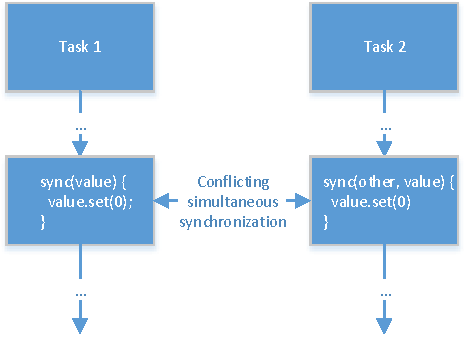
\includegraphics[scale=.9]{pics/ParallelExecutionAttempt}
\end{minipage}
}
\begin{minipage}{0.2\textwidth}
\begin{center}
\vspace{3.5cm}
$\longrightarrow$

actual execution
\end{center}
\end{minipage}
\adjustbox{valign=t}{
\begin{minipage}{0.4\textwidth}
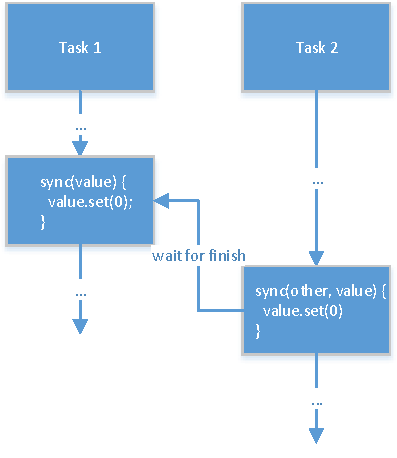
\includegraphics[scale=.9]{pics/SerialExecution}
\end{minipage}}

The possibility to refer to multiple shared resources in the synchronization list of a synchronization statement is not mere syntactic sugar for nested synchronization statements. Instead, the semantics of a synchronization list are that all referenced shared resources are synchronized over at once, but with a possible time delay. By the design of the underlying implementation deadlocks by competing synchronization statements are thus avoided.\footnote{Nevertheless, deadlocks can obviously still occur if nested synchronization statements compete for the same resources in an unsorted order.}

As a result of the fact that generally the access to shared resources is resource-centric, a value wrapped in a shared resource which in turn contains nested shared resources is independently protected from the latter. Therefore, a shared resource of a struct with a shared member \CODE{b} is independently synchronized from \CODE{b}:

\vspace{0.5cm}
\begin{minipage}{0.35\textwidth}
\begin{ccode}
struct A {
  int32 a;
  shared<int32> b; 
}
shared<A> sharedA;
shared<int32>* sharedB;
sync(sharedA) { sharedB = &(sharedA.get.b); }
\end{ccode}
\end{minipage}
\begin{minipage}{0.2\textwidth}
\begin{center}
\end{center}
\end{minipage}
\begin{minipage}{0.35\textwidth}
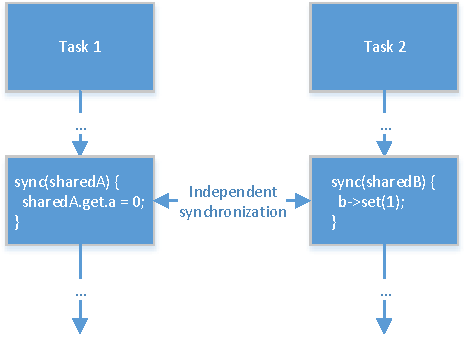
\includegraphics[scale=.9]{pics/ParallelExecution}
\end{minipage}

The translation of shared resources is currently only supported for executable programs. Therefore, it is not safe to use shared types and synchronization statements in libraries that are written with mbeddr. The explanations of the following section are therefore focused to according scenarios, although the translation for library code would only change in details.

\subsection{Translation of shared types}
\label{sharedTypesTranslation}
In order to fully understand the translation of synchronization statements, the translation of shared types is given first. For the implementation of shared types in C, two main solutions are conceivable, which differ in the coupling that they exhibit between the data that is to be shared and the additional data required for access restriction, i.e. synchronization. In any case, a solution must make use of additional data that can be used to synchronize two threads which try to read or write the shared data. To this end, the most basic synchronization primitive was chosen: each protected data item is assigned exactly one mutex. 

In the first solution, the data to be shared is stored as if no protection scheme existed at all. Additionally, all mutexes that are created by the application are stored in one global map, which indexes each mutex by the memory address of its corresponding shared datum. This approach offers the advantage that access to the data itself is not influenced by the mutex protection: Every reference to the value of a shared resource \CODE{e.get} can directly be translated into a reference to the wrapped value. Additionally, since the mutexes are globally managed, all data that is returned by a library can be easily made (pseudo-) synchronization safe. For instance, if a pointer to an arbitrary memory location \texttt{loc} is returned, the pointed-to address can be used to create a new mutex and add a mapping to the global mutex map. However, this on-the-fly protection of memory locations can incur synchronization leaks: The compiler cannot guarantee that addresses returning functions with unknown implementation will not leak their returned values to some other computation which accesses the according memory unsynchronized. This implies that such protection would only be safe if any reference to \texttt{loc} was wrapped in some shared resource which, in this scenario, is not feasible. Hence, a design was chosen that does not allow for such protection. Consequently, a global map would not be beneficial in this regard. A map solution would entail a space-time trade-off. For instance, Google's C++ \textit{dense\_hash\_map}, \footnote{http://goog-sparsehash.sourceforge.net/doc/dense\_hash\_map.html} provides comparatively fast access to its members but imposes additional memory requirements in comparison to slower hash map implementations\footnote{See http://incise.org/hash-table-benchmarks.html for details. This examplary library should be considered as an illustrative example for the general space-time trade-off that is inherent with maps.}. A disadvantage of hash maps is the non-deterministic performance\footnote{Although real-time applications with their time-wise constraints are not a primary concern of this work, it should nevertheless be kept in mind that they are part of the embedded domain. Therefore, a solution that considers the characteristics of this domain is at least regarded advantageous.} and increased access time that may be induced by hash collisions \cite{FastAndDeterministicHashTable}.

The second solution for the implementation of shared types keeps each shareable datum and its mutex together. An instance of a struct with member fields for both components is used in place of the bare datum to be shared. In contrast to the aforementioned solution, a reference to the value \CODE{e.get} needs one level of indirection via the struct instance. However, the access to a mutex is simplified. As with the value, it can be retrieved by a member access to the corresponding struct field, whereas the map solution requires a map lookup to get the mutex (plus additional delay to make any modifying access to the map thread-safe). The computational overhead imposed by a struct member lookup is deemed negligible in the overall application performance. On the other hand, the space required for the struct equals that of the individual fields plus additional padding \cite[pp.~303 ff.]{LinuxSystemProgramming} that is required to arrange the struct fields along valid memory addresses. The latter depends on the size of the data to be stored. In order to keep the padding as small as possible, smart member ordering should be applied. 

For this work, the struct solution was chosen in order to keep the access time of mutex lookups small and deterministic while not imposing too much space overhead and datum lookup overhead. For each kind of shared type \CODE{shared<t>} with the translated base type \CODE{t'} a separate struct is generated:
\begin{ccode}
struct SharedOf_t {
  pthread_mutex_t mutex;
  t' value;
}
\end{ccode}
Any nested shared types are, hence, translated first. For implementation reasons nested \textit{typedef}s and constants used in array types are also resolved in this process.\footnote{Although the resolution of typedefs and constants impedes corresponding (test-wise) adjustments made by the programmer in the translated C code, this is not deemed an issue since generally changes should always be made from within mbeddr, i.e. on the original code.} Depending on the base type of the shared type, the generated struct declaration is stored either in a generic module or in a newly generated other module. Consider the tree for a type \CODE{shared<t>} whose nodes are made of types and whose edges are formed by the base type relationship of shared types, array types and pointer types,\footnote{Clearly, this tree will have only one branch.} e.g: 


\begin{minipage}{0.3\textwidth}
\begin{ccode}
struct A { int32 val; }
shared<shared<A[10][20]>*>
\end{ccode}
\end{minipage}
\begin{minipage}{0.3\textwidth}
\begin{center}
\quad$\longrightarrow$\qquad

the simplified type AST
\end{center}
\end{minipage}
\begin{minipage}{0.5\textwidth}
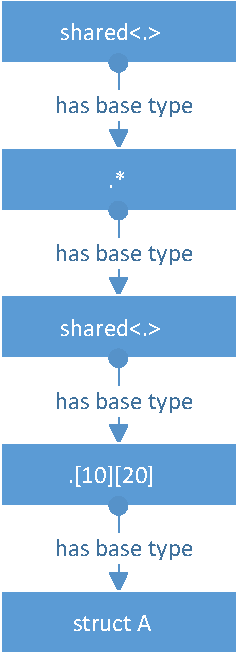
\includegraphics[scale=0.7]{pics/AstForBaseTypes}
\end{minipage}

\vspace{0.5cm}
If the leave of the tree is a primitive C type the struct declaration is stored in a generic module. In any other case the leave must be some struct type \CODE{s}. In order to preserve the visibility of the corresponding struct in the newly generated struct \CODE{SharedOf\_t}, the latter is stored in the same module. Since the generation of code related to shared types can diminish the legibility of the resulting code profoundly for every such module, a specific \textit{SharedTypes\_X} module is created and imported into the module that declares \CODE{s}. \textit{SharedTypes\_X} is used to store struct declarations like \CODE{SharedOf\_t}. Furthermore \CODE{s} is lifted into it in order to make it visible in the member declaration \CODE{value} of \CODE{SharedOf\_t}. For any field of \CODE{s} whose type tree contains another user-defined struct type, the corresponding struct declaration is either lifted, as well (and recursively treated in the same way) or imported by its module. Should this separation of generated code used for shared type declarations and other user-defined code not proof well in praxis, it could easily be deactivated.
With the former generation of the struct declaration in mind a type \CODE{shared<t>} is reduced to:
\begin{ccode}
SharedOf_t
\end{ccode}
The reduction of an expression \CODE{e.get} and \CODE{e.set(f)} make use of the \CODE{value} field of the \CODE{SharedOf\_t} struct. They are basically reduced to a retrieval of, respectively an assignment to the field:

\begin{minipage}{0.15\textwidth}
\begin{ccode}
e'.value
\end{ccode}
\end{minipage}
\begin{minipage}{0.2\textwidth}
respectively
\end{minipage}
\begin{minipage}{0.3\textwidth}
\begin{ccode}
e'.value = f'
\end{ccode}
\end{minipage}

If \CODE{e'} has a pointer type, the expressions \CODE{e->get} and \CODE{e->set(f)} are reduced to:

\begin{minipage}{0.15\textwidth}
\begin{ccode}
e'->value
\end{ccode}
\end{minipage}
\begin{minipage}{0.2\textwidth}
respectively
\end{minipage}
\begin{minipage}{0.3\textwidth}
\begin{ccode}
e'->value = f'
\end{ccode}
\end{minipage}

The mutex of the struct \CODE{SharedOf\_t} in the equally named struct field \CODE{mutex}, which is used to synchronize one variable of an according type, must be initialized prior to any usage. This is done implicitly by generated code, in order to free the programmer from this task. Accordingly, mutexes must be released before they get out of scope to prevent memory leaks. In the generated code, both functionalities make use of corresponding functions, i.e. for every type who is one of the following types a pair of \CODE{mutexInit}--\CODE{mutexDestroy} functions is generated:

\begin{itemize}
\item shared types whose base types are shared types or for whom mutex functions are recursively generated;
\item array types which are not base types of array types themselves and whose base types are either shared types or struct types for whom mutex functions are recursively generated;
\item struct types whose structs contain at least one field with a type for which the same relation holds as for the aforementioned types.
\end{itemize}

For example, a type \CODE{shared<int32>[42][24]} would enforce the generation of one mutex initialization and one mutex destruction function. \CODE{shared<int32>*} on the other hand would not. Any variable \CODE{v} of the latter type would point to a shared ressource which must be referenced directly by another variable \CODE{v'} of type \CODE{shared<int32>} or be contained in the memory-addressable value of some variable \CODE{v''} of a more complex type. The declaration of \CODE{v'}, respectively \CODE{v''}, would then trigger the initialization of the mutex of the shared resource that \CODE{v} points to. The resulting mutex initialization functions for types of the aforementioned kind are declared as follows:

\begin{ccode}
// for a proper shared type shared<t> and the type t' that t is reduced to
void mutexInit_X(SharedOf_t'* var) { 
  pthread_mutex_init(&var->mutex, &mutexAttribute);
  
  // either if t is a shared type or a struct type:
  mutexInit_X'(&var->value); 
  
  // or if t is an array type t[i_1]...[i_n] of 1 to n dimensions:
  mutexInit_X'((SharedOf_t'*...*)var->value, i_1, ..., i_n); 
}
\end{ccode}
For a shared resource, first the mutex of the corresponding translated struct is initialized by a call to the POSIX function \CODE{pthread\_mutex\_init()}, which takes a mutex pointer and a mutex attribute pointer.\footnote{The meaning of the mutex attribute will be explained later on.} Then -- since by aforementioned conditions the shared resource contains another shared resource -- a call to the appropriate mutex function for the contained value is triggered. Depending on whether the base type of the current shared type is an array additionally the dimension sizes for this base type may need to be provided as well (see below for details).

\begin{ccode}
// for a proper array type t[]...[] of 1 to n dimensions where ... denotes the occurrence of accordingly many symbols 
// and t' denotes the reduced-to type
void mutexInit_X(t'*...* var, int32 size_0, ..., int32 size_n) { 
  for (int32 __i_0 = 0; __i_0 < size_0; __i_0++) { 
    ...
      for (int32 __i_n = 0; __i_n < size_n; __i_n++) {
        // in case t is a struct type
        mutexInit_X'(&var[__i_0]...[__i_n]);
        
        // or, in case t is a shared type with generic C base type:
        pthread_mutex_init(&var[__i_0]...[__i_n].mutex, &mutexAttribute);
      }
    ...
  } 
}
\end{ccode}
For shared ressoures that are nested in arrays, a nested iteration over all elements of the corresponding possibly multidimensional array with calls to either the generated mutex functions or the function defined by the POSIX standard are triggered.

For structs with nested shared resources for each field that is or contains a shared resource, either the \CODE{pthread\_mutex\_init()} function is called directly or the mutex initialization is done by a call to the already generated function that is type compatible with this field (by possibly providing additional array dimensions):

\begin{ccode}
// for a proper struct type t of a struct t { u_1 f_1; ...; u_n f_n } and according reduced field types u_1' to u_n'
void mutexInit_X(SharedOf_t* var) {
  ...
  // in case u_i demands further initialization and it is a struct type or a shared type
  mutexInit_X'(&var->f_i);
  
  // in case u_i demands further initialization and is an array type u_i[j_1]...[j_n] of 1 to n dimensions:
  mutexInit_X'((SharedOf_u_i'*...*)var->f_i, j_1, ..., j_n);
  
  // or, in case u_i is a shared type with a generic C base type:
  pthread_mutex_init(&var->f_i.mutex, &mutexAttribute);
  ...
}
\end{ccode}
The signature of \CODE{mutexInit\_X()} for arrays shows that those are not passed as arrays to the mutex functions, but as pointers. This is due to the necessity of declaring multidimensional arrays at least partially with the size for each dimension (e.g. \CODE{int[][]} would be missing at least one dimension size). Nevertheless it would not make sense to declare one mutex function for each shape of dimension size. Since arrays are treated like pointers internally when they are passed as function arguments, it is completely safe to cast them to appropriate pointer types and to use equal types for the according function parameters.

The deletion of mutexes is defined quite similar to the initialization, with the main difference that the utilized according pthreads function only takes one mutex. Therefore, only the deletion of mutexes nested in resources of shared types is shown:
\begin{ccode}
void mutexDestroy_X(SharedOf_t'* var) { 
  pthread_mutex_destroy (&var->mutex); 
  // ... further call to a mutexDestroy_X function equivalently to mutexInit_X shown above
}
\end{ccode}
The presented functions are used to initialize mutexes at the beginning of their life span and delete them right before the corresponding end. For mutexes refered to by global variables this means that they must be initialized at the beginning of the entry function of the program.\footnote{Due to the way mutexes are used in ParallelMbeddr (recursively and nested in structs -- as will be shown in the following paragraphs) and the peculiarities of C and the POSIX standard, there is no way to combine the definition and the initialization of mutexes.} As already forced for executable programs by mbeddr, the programmer thus has to specify a main function. Similarly, mutexes of local variables are initialized right after their declaration, whereas mutexes of function arguments are declared at the beginning of the related function.\footnote{\label{mutexCopies}It is not an obvious choice to enable the programmer to use function arguments which contain or are shared resources and: C's pass-by-value semantics of function parameters causes parameters to be copied into functions. Therefore, a shared resource which is not passed by its addresses but by its actual value will provoke the generation of an equal shared resource at the beginning of the function execution. This copy is synchronization-wise completely unrelated to the original shared resource, since mutex copies cannot be used to lock with their origins \cite{Mutexes}. Furthermore, they have to be initialized and destroyed separately. The use of shared resources in such a manner can confuse programmers who are not aware of this fact. Nevertheless ParallelMbeddr allows this kind of utilization of shared resources in order to not burden the programmer with having to copy large structs that contain shared resources component-wise if the shared resource data is not of relevance. Depending on the feedback of future users, it should be considered whether warnings for unintended misuse of shared resources in this way might be helpful.} The deletion of mutexes for shared resources must be accomplished before they get out of scope which, again, depends on the kind of variables they are referred to. 

Mutexes for global variables need not be destroyed at all in order to avoid memory leaks. Their lifetimes span the whole program execution so that the  memory allocated to these mutexes will be cleaned up by the underlying operating system. On the other hand, the mutexes of local variables must be destroyed before they get out of scope. Hence, mutex destruction calls are added at the end of the surrounding scopes of mutexes. If control flow breaking statements (\textit{return}, \textit{break}, \textit{continue}, \textit{goto}) are present, additional calls are inserted according to the following rules. Take any control-flow-breaking statement \textit{c} that occurs in the AST of the same function as the declaration \textit{l} of some local variable, which refers to a (nested) shared resource. If \textit{c} is part of the AST of any statement that follows \textit{l}\footnote{In other words: Consider only those control-flow-breaking statements \textit{c}s that are either one of the statements \textit{stmt}s which have the same AST parent \textit{p} and follow \textit{l} in the statement list of \textit{p} or are contained in the AST of some \text{stmt}} and
\begin{itemize}
\item \textit{c} is a \textit{return} statement and refers to a function or a closure whose AST contains \textit{l} or
\item \textit{c} is a \textit{break} statement and refers to a loop or a \textit{switch} statement case whose AST contains \textit{l} or
\item \textit{c} is a \textit{continue} statement and refers to a loop whose AST contains \textit{l} or
\item \textit{c} is a \textit{goto} statement and refers to a label outside the AST of any statement that follows \textit{l}.
\end{itemize}
\textit{c} must be preceded with a destruction call of the mutex of the shared resource of \textit{l} (compare with the synchronization stopping rules below). Allocated memory that is not freed at the end of the program is automatically released by the operating system. Hence, a \textit{return} statement that refers to the entry function of the program need not be preceded with destruction calls of its local shared resources. The proper destruction of a mutex of an argument of function \textit{f} just requires according function calls at the end of \textit{f} and before any return statement that refers to \textit{f}. 

As inside the declarations of the mutex destruction functions explained above, the actual function to call for a variable or argument is either one of the \CODE{mutexDestroy\_X()} functions or a direct call of \CODE{pthread\_mutex\_destroy()} for `simple' shared resources of generic C types, e.g.:
\begin{center}
\begin{minipage}{0.3\textwidth}
\begin{ccode}
// simple shared resource
shared<int32> v1;

// complex shared resource
shared<int32>[2][3] v2;
\end{ccode}
\end{minipage}
\qquad$\Longrightarrow$\qquad\qquad
\begin{minipage}{0.4\textwidth}
\begin{ccode}
SharedOf_int32_0 v1;
pthread_mutex_init(&v1.mutex, &mutexAttribute);

SharedOf_int32_0[2][3] v2;
mutexInit_0((SharedOf_int32_0**)v2, 2, 3);
\end{ccode}
\end{minipage}
\end{center}

To recap: The mutex of a shared resource is either directly initialized and destroyed via appropriate pthreads functions or it is indirectly handled via functions that are based on the types of the values that shared resources are nested in. This approach was chosen in order to reduce the amount of code duplication that would occur if mutexes of shared resources would be handled inline for every according variable. As a result the generated code's readability is enhanced. The additional computational overhead due to function calls and returns should be regarded as an optimization concern of a further compilation step by a compiler like \textit{gcc}.

ParallelMbeddr does not prevent the programmer from structuring the synchronization statements in such a way that a task will synchronize a shared variable multiple times (\textit{recursive synchronization}). The following code depicts such behavior:
\begin{ccode}
shared<int32> sharedValue;
sync(sharedValue) {
  sync(sharedValue) {
    sharedValue.set(42);
  }
}
\end{ccode}
Since each synchronization statement locks the mutexes of the refereed shared resources (see below for details), a recursive synchronization results in a \textit{recursive lock} of the corresponding mutex. Mutexes as defined by the POSIX standard must be specifically initialized in order to allow for this behavior:\footnote{By default a recursive lock results in undefined behaviour because a default mutex does not have a lock count which is required to make recursive locks work: http://linux.die.net/man/3/pthread\_mutex\_trylock.} A mutex attribute that specifies the recursiveness must be defined and initialized first. It can then be used by arbitrarily many mutexes. For this purpose, an application-wide attribute is defined in a generic module that is imported by all user-defined modules. It is initialized at the beginning of the main function:
\begin{ccode}
// inside the generic module:
pthread_mutexattr_t mutexAttribute
// at the beginning of main:
pthread_mutexattr_init(&mutexAttribute);
pthread_mutexattr_settype(&mutexAttribute, PTHREAD_MUTEX_RECURSIVE);
\end{ccode}

\subsection{Translation of synchronization statements}
Every synchronization statement is reduced to its statement list -- as a block --, surrounded with calls to functions that control the synchronization of the mutexes. The reduction of such a statement is given either by

\begin{center}
\begin{minipage}{0.3\textwidth}
\begin{ccode}
sync(e) stmt_list
\end{ccode}
\end{minipage}
\qquad$\Longrightarrow$\qquad\qquad\qquad
\begin{minipage}{0.4\textwidth}
\begin{ccode}
startSyncFor1Mutex(&e.mutex);
stmt_list'
stopSyncFor1Mutex(&e.mutex);
\end{ccode}
\end{minipage}
\end{center}

in case it contains only one synchronized resource, or else by

\begin{center}
\begin{minipage}{0.3\textwidth}
\begin{ccode}
sync(e_1, ..., e_n) stmt_list
\end{ccode}
\end{minipage}
\qquad$\Longrightarrow$\qquad\qquad\qquad
\begin{minipage}{0.4\textwidth}
\begin{ccode}
startSyncForNMutexes(&e_1.mutex, ..., &e_n.mutex);
stmt_list'
stopSyncForNMutexes(&e_1.mutex, ..., &e_n.mutex);
\end{ccode}
\end{minipage}
\end{center}

The statements are kept inside their statement list block in order to keep the scope of local variables inside synchronization statements. A synchronization statement list block is reduced to another block where statements that break the program flow structure may be preceded by an identical call of the \CODE{stopSyncForNMutexes()} function as is present after the list: Let \textit{s} be a synchronization statement and \textit{c} be a control-flow-breaking statement which is nested on some level in the AST of \textit{s}' statement list. Then \textit{c} is preceded with a call to \CODE{stopSyncForNMutexes()} if one of the following cases holds:
\begin{itemize}
\item \textit{c} is a \textit{return} statement and refers to a function or a closure whose AST contains \textit{s};
\item \textit{c} is a \textit{break} statement and refers to a loop or a \textit{switch} statement case whose AST contains \textit{s};
\item \textit{c} is a \textit{continue} statement and refers to a loop whose AST contains \textit{s};
\item \textit{c} is a \textit{goto} statement and refers to a label outside the AST of \textit{s}.
\end{itemize}

In this manner, inconsistent synchronization states of shared resources due to a control flow break by the aforementioned statements are omitted. Since the occurrence of such a statement may also force ParallelMbeddr to insert \CODE{mutexDestroy\_X()} calls, a careless mixture of mutex unlocking and destruction calls can cause runtime errors \cite{Mutexes}. The generator therefore ensures that any destruction calls are put behind the generated unlocking calls.

For each arity of synchronization resources, separate versions of the \CODE{start}- and \CODE{stopSyncForNMutexes()} functions are declared inside a generic C module. A \CODE{stopSyncForNMutexes()} function straightforwardly redirects its mutex parameters to calls of the \CODE{pthread\_mutex\_unlock} function:
\begin{ccode}
// the corresponding function 'stopSyncFor1Mutex()' for exactly one mutex is skipped here
void stopSyncForNMutexes(pthread_mutex_t* mutex_1, ..., pthread_mutex_t* mutex_n) { 
  pthread_mutex_unlock (mutex_1);
  ...
  pthread_mutex_unlock (mutex_n); 
}
\end{ccode}

Abstracted over the details of the actual implementation, synchronization statements synchronize their ressources atomically, as was mentioned in the preceding design section. Since one or more mutexes can be tentatively locked by multiple threads simultaneously, specific contention management has to be taken care of. The illusion of atomic synchronization is realized by an implementation of the obstruction-free\footnote{Busy-waiting means that the thread will repeatedly test a condition until it is met, without doing actual useful work \cite[p.~166]{AnIntroductionToParallelProgramming}. Thus, it is an alternative to suspending a thread and revoking it later on when some condition is met (which can, e.g., be realized by \textit{condition variables} as provided by POSIX threads \cite[p.~77]{ProgrammingWithPOSIXThreads}). Obstruction-free means that the execution of any thread will progress when at some time the thread is run in isolation, i.e. when the execution of obstructing other threads is interrupted meanwhile. The existence of obstruction-freedom guarantees that no deadlocks will occur \cite{ObstructionFreeAuthorizationEnforcement}. However, livelocks and starvation are not necessarily avoided. Stronger degrees of non-blocking algorithms like lock-freedom and wait-freedom tackle these problems (partially), but are not relevant for this work. Further information on the latter is for instance provided by http://preshing.com/20120612/an-introduction-to-lock-free-programming/. %http://doc.akka.io/docs/akka/snapshot/general/terminology.html
} busy-wait protocol \textit{Polite}. In order to resolve conflicts, \textit{Polite} uses exponential back-off. The according back-off function is explained further down. The synchronization function tries to lock every mutex as given by its arguments. On failure, it releases every mutex that was locked so far, uses the back-off function to delay its execution for a randomized amount of time, and repeats afterwards. This scheme enables competing threads to (partially) proceed and avoid deadlocks due to unordered overlapping mutex locks.\footnote{Again, the presented scheme does not prevent the programmer from nesting the synchronization statements in such a manner that deadlocks in nested synchronization statements occur. It is rather a prevention of deadlocks that are caused solely by synchronization statements on the same nesting level.}
\begin{ccode}
// again, the equivalent function declaration for one mutex is skipped
void startSyncForNMutexes(pthread_mutex_t* mutex_0, ..., pthread_mutex_t* mutex_m, pthread_mutex_t* mutex_n) { 
  uint8 waitingCounter = 0; 
  uint16 mask = 16; 
  uint32 seed = (uint32)(uintptr_t) &waitingCounter;
  
  while (true) { 
    if ([| pthread_mutex_trylock (mutex_0) |] != 0) { 
      backoffExponentially(&waitingCounter, &mask, &seed); 
    } 
    else if ([| pthread_mutex_trylock (mutex_1) |] != 0) { 
      [| pthread_mutex_unlock (mutex_0) |]; 
      backoffExponentially(&waitingCounter, &mask, &seed); 
    } ...
    else if ([| pthread_mutex_trylock (mutex_n) |] != 0) { 
      [| pthread_mutex_unlock (mutex_m) |];
      ...
      [| pthread_mutex_unlock (mutex_0) |]; 
      backoffExponentially(&waitingCounter, &mask, &seed); 
    } 
    else { 
      break; 
    } 
  }
}
\end{ccode}

The back-off realized by Polite delays the execution  by less than \textit{limit} $ = 2^{n+k}$ ns \cite{AdvancedContentionManagement} in a randomized fashion. \textit{n} denotes the retry counter and \textit{k} denotes some constant offset which can be machine-tuned. The randomized wait time of the exponential back-off is used to avoid livelocks which could happen if two threads would repeatedly compete for the same resources and delay their execution for equal amounts of time. In the current implementation \CODE{backoffExponentially()} of the contention management, the offset \textit{k} is set to 4 and a threshold \textit{m} of 17 denotes the number of rounds after which \textit{k} is reset.\footnote{\textit{k}'s value is reflected in the initial value ($2^4 = 16$) of \CODE{mask} whereas \textit{m}'s value is composed of mask's base and the divisor (13) in the calculation of the next \CODE{waitingCounter}.} Thus, maximum delays of about 100 ms (specifically 131 ms) are allowed.\footnote{The search for machine- or application-specific optimal offsets and thresholds is a task for future enhancements of ParallelMbeddr.}
\begin{ccode}
inline void backoffExponentially(uint8* waitingCounter, uint16* mask, uint32* seed) { 
  *mask |= 1 << *waitingCounter; 
  randomWithXorShift(seed); 
  struct timespec sleepingTime = (struct timespec){ .tv_nsec = *seed & *mask }; 
  nanosleep(&sleepingTime, null); 
  *waitingCounter = (*waitingCounter + 1) % 13; 
}
\end{ccode}
It has to be noted that \CODE{backoffExponentially()} keeps its main state inside the \CODE{startSyncForNMutexes()} function. The state will therefore be re-initialized before the execution of every synchronization block. The generation of the pseudo-randomized delay is realized via utilization of the Marsaglia's Xorshift random number generator \cite{XorshiftRngs}:
\begin{ccode}
void randomWithXorShift(uint32* seed) { 
  *seed ^= *seed << 13; 
  *seed ^= *seed >> 17; 
  *seed ^= *seed << 5; 
}
\end{ccode}
The generator was chosen for its high performance, low memory consumption, and thread safety due to the utilization of the stack-managed \CODE{seed} parameter as opposed to the global state usage of the standard C random generator \CODE{rand()}. The fact that after a certain number -- which may be smaller than in other generators -- of repeated calls with the same seed value (i.e. the same memory address of a seed) repetitions of the sequence of calculated numbers will occur is not of relevance for the purpose of this work.

\subsection{Example code}
\label{sharedMemoryExample}
In the previous sections \ref{taskExample} and \ref{futuresExample} the running example approximated the number $\pi$ by using tasks which calculate exactly one fraction of the result each and by retrieving their results via futures. The amount of work was therefore partitioned in advance. In this section, a more dynamic approach is chosen instead: The work of every task comprises major and minor rounds. A minor round is equivalent to the full calculation loop in the previous $\pi$ solution. In every step of a major round, a minor round is initiated by first coordinating with the other tasks which range of $\pi$ the current task should calculate. After having calculated the sum in a minor round, the task then uses a queue to store its next partial result. A dedicated task is used to collect these partial results from the queue and accumulate them to a complete sum, which eventually becomes the result of the over-all approximated $\pi$. The communication-based solution can be seen as a map-reduce implementation where partial results are mapped onto the queue by a certain number of tasks and from there reduced to a final result by a separate task (compare with \cite{MapReduce}).
In order to understand the new implementation, first it has to be considered that a thread-safe queue of a certain size and slots of type \CODE{long double} is given as a black box. Further suppose that functions for the initialization, for adding a value and getting the next value (or wait for the next value), exist:
\begin{ccode}
struct Queue {...}
void queueInit(shared<Queue>* queue);
void queueSafeAdd(shared<Queue>* queue, long double item);
void queueSafeGet(shared<Queue>* queue, long double* result);
\end{ccode}
As in the previous approach, the amount of work to be done is defined by a range size (number of minor task rounds) and the number of ranges altogether. Additionally, the number of mapper tasks is set to a certain value that should be in the order of the number of processors:
\begin{ccode}
#constant RANGESIZE = 300000000; 
#constant RANGECOUNT = 4; 
#constant THRESHOLD = RANGESIZE * RANGECOUNT; 
#constant MAPPERCOUNT = 2;
\end{ccode}
These constants are used to initialize the mappers and the reducer in the main function appropriately:
\begin{ccode}
exported int32 main(int32 argc, string[] argv) { 
  shared<Queue> queue; 
  queueInit(&queue); 
  shared<Queue>* queuePointer = &queue; 
   
  shared<uint32> counter; 
  shared<uint32>* counterPointer = &counter; 
  sync(counter) { counter.set(0); } 

  Task<void> mapperTask = |map(THRESHOLD, counterPointer, queuePointer)|; 
  Future<void>[MAPPERCOUNT] mappers; 
  for (i ++ in [0..MAPPERCOUNT[) { 
    mappers[i] = mapperTask.run; 
  }
  mapperTask.clear;
   
  shared<long double> result; 
  shared<long double>* resultPointer = &result; 
   
  |reduce(RANGECOUNT, resultPointer, queuePointer)|.run.join;
  
  return 0; 
}
\end{ccode}

First the queue is defined as being shared in order to be accessible by all tasks. After the initialization, a pointer to the queue is created, which is necessary since any other reference inside a task expression to the queue variable would otherwise cause a copy of the queue struct instance into the task, regardless of whether later on the address of the referred value is retrieved via the \CODE{\&} operator. This `shortcoming' of the current semantics could be addressed by the introduction of a new address operator that creates a temporary variable of the addressed value and should be considered for future extensions of ParallelMbeddr. Similar to the queue, a \CODE{counter} variable is introduced which will be used by the tasks to check and communicate how many ranges have been processed so far. Then, one mapper task is defined and initialized with a task expression of a call to the \CODE{map()} function. For communication purposes, the mapper gets the queue pointer and the counter pointer. Additionally, although due to the use of constants not necessary in the current example, the mapper task is told the maximum number of items that need to be calculated. This single task template\footnote{\CODE{mapperTask} can be seen as a template for actual running mapper task instances.} is used to create multiple running tasks and store their handles as futures in a \CODE{mappers} array. The reducer uses a pointer to a result value memory location to safe its result. Further, it gets access to the queue via a pointer thereof and is told how many items (\CODE{RANGECOUNT}) it shall read from the queue before termination. The code shows the first example of a task expression chain: First the task is declared, then an instance of it is run in parallel and immediately the main task joins the reducer. Since nothing is done in the main task between the run and the join, the serialized execution could also be realized by a simple function call to \CODE{reduce()}. For demonstrative purposes, the code was chosen this way nevertheless. The main task solely joins the reducer task, since after its termination every mapper task will also be finished.
The \CODE{map()} function iteratively calculates complete ranges of fractions of $\pi$ until the maximum number of items as given by \CODE{threshold} is reached:
\begin{ccode}
void map(uint32 threshold, shared<uint32>* counter, shared<Queue>* resultQueue) { 
  while (true) { 
    uint32 start; 
    uint32 end; 
     
    sync(counter) { 
      start = counter->get; 
      if (start == threshold) { 
        break; 
      } 
      uint32 possibleEnd = start + RANGESIZE; 
      end = (possibleEnd <= threshold)?(possibleEnd):(threshold); 
      counter->set(end); 
    } 
     
    queueSafeAdd(resultQueue, calcPiBlock(start, end)); 
  } 
}
\end{ccode}
In every iteration, the function synchronizes the shared resources that \CODE{counter} points to in order to retrieve its value and increment it by the number of items that \CODE{map()} is going to calculate in the current round. It uses the \CODE{calcPiBlock()} function that was presented in section \ref{taskExample} to calculate a partial sum. Afterwards, the result is added to the queue. 
The \CODE{reduce()} function uses the queue to iteratively read all partial results and update the value of the shared resource of the final result accordingly:
\begin{ccode}
void reduce(uint32 numberOfItems, shared<long double>* finalResult, shared<Queue>* partialResultQueue) {
  sync(finalResult) { 
    for (uint32 i = 0; i < numberOfItems; ++i) { 
      long double item; 
      queueSafeGet(partialResultQueue, &item); 
      finalResult->set(item + finalResult->get); 
    }
  }
}
\end{ccode}
During the whole calculation, \CODE{reduce()} synchronizes the result variable in order to keep the synchronization overhead small. It is able to do this because no other task will try to access the result before the termination of the single reducer task.

In the beginning of the translated main function, the global mutex attribute is initialized, which will be reused for every mutex. Afterwards, the declared queue is initialized:
\begin{ccode}
pthread_mutexattr_settype(&mutexAttribute_0, PTHREAD_MUTEX_RECURSIVE); 
pthread_mutexattr_init(&mutexAttribute_0); 
initAllGlobalMutexes_0(); 
SharedOf_Queue_0 queue; 
mutexInit_2(&queue); 
queueInit(&queue); 
SharedOf_Queue_0* queuePointer = &queue;
\end{ccode}
The translated struct type \CODE{SharedOf\_Queue\_0} of the original type \CODE{shared<Queue>} refers to a struct that contains a field for the protected queue and a mutex field:
\begin{ccode}
struct SharedOf_Queue_0 { 
  pthread_mutex_t mutex; 
  Queue value; 
};
\end{ccode}
The mutex initialization function \CODE{mutexInit\_2()} initializes the mutex of the shared queue and calls another initialization function which in turn initializes any nested mutexes of the \CODE{Queue} struct. Similarly, a destruction function is generated:
\begin{ccode}
void mutexInit_2(SharedOf_Queue_0* var) { 
  pthread_mutex_init(&var->mutex, &mutexAttribute_0); 
  mutexInit_1(&var->value); 
}
void mutexDestroy_2(SharedOf_Queue_0* var) { 
  pthread_mutex_destroy(&var->mutex);
  mutexDestroy_1(&var->value); 
}      
\end{ccode}
Similar to the declarations for the queue, the mbeddr generator creates declarations of a struct for the \CODE{result} variable. The initialization and destruction of \CODE{result} is accomplished inline by calls to the pthreads functions, since no nested mutexes for the fields of the struct exist:
\begin{ccode}
struct SharedOf_long_double_0 { 
  pthread_mutex_t mutex; 
  long double value; 
};
... // in main()
SharedOf_long_double_0 result; 
pthread_mutex_init(&result.mutex, &mutexAttribute_0); 
SharedOf_long_double_0* resultPointer = &result;
\end{ccode}
Lastly, the \CODE{counter} variable shows how translated shared resources can be synchronized.\footnote{The declarations of the struct and the mutex functions for the \CODE{counter} variable are skipped.} For the duration of the setting of \CODE{counter}'s value, its mutex is locked. The setting of the value is done by an assignment to the \CODE{value} field of the generated struct that keeps the value of the shared resource:
\begin{ccode}
SharedOf_uint32_0 counter; 
pthread_mutex_init(&counter.mutex, &mutexAttribute_0); 
SharedOf_uint32_0* counterPointer = &counter;

startSyncFor1Mutex(&counter.mutex); 
{ counter.value = 0; } 
stopSyncFor1Mutex(&counter.mutex);
\end{ccode}

The mutexes of all shared resources are destroyed at the end of the main function. Although this should not be necessary for local variables of the entry function of the program, the compiler currently does not distinguish between the main function and any other function for which such calls would be necessary\TODO{maybe fix this}:
\begin{ccode}
mutexDestroy_2(&queue); 
pthread_mutex_destroy(&counter.mutex); 
pthread_mutex_destroy(&result.mutex);
\end{ccode}
The initializations of the tasks and the declarations of the futures is quite similar to those in section \ref{taskExample}:
\begin{ccode}
Task mapperTask = taskInit_0(queuePointer, counterPointer);
// mappers:
VoidFuture[MAPPERCOUNT] mappers; 
for (int8 __i = 0; __i < MAPPERCOUNT; __i++) { 
  mappers[__i] = runTaskAndGetVoidFuture(mapperTask); 
}
free(mapperTask.args);

// reducer:
saveAndJoinVoidFuture(futureInit_0(resultPointer, queuePointer));
\end{ccode}

Since in the new solution the tasks do not return any results directly, the \CODE{VoidFuture} struct and respective functions are used. For the lack of valuable new insight the declarations of the \CODE{taskInit\_0()} function and \CODE{Args\_X} structs is skipped, here. Instead recall the original code \CODE{|reduce(RANGECOUNT, resultPointer, queuePointer)|.run.join}. As was shown in section \ref{futuresTranslation} the run call and the task declaration are reduced to a call of a function which combines the intialization of a task with the one of a future of a parallel running instance of this task. This call is reflected by \CODE{futureInit\_0(resultPointer, queuePointer)}. Furthermore the join of the task must first bind the created future handle to some addressable location before it can use this handle by its address. For this reason \CODE{saveAndJoinVoidFuture} is used in place of \CODE{joinVoidFuture}. The declaration of \CODE{futureInit\_0} follows:
\begin{ccode}
VoidFuture futureInit_0(SharedOf_long_double_0* resultPointer, SharedOf_Queue_0* queuePointer) { 
  Args_1* args_1 = malloc(sizeof(Args_1)); 
  args_1->resultPointer = resultPointer; 
  args_1->queuePointer = queuePointer; 
  pthread_t pth; 
  pthread_create (&pth, null, :parFun_1, args_1) |]; 
  return (VoidFuture){ .pth = pth }; 
}
\end{ccode}
The original declaration of the reducer task contains references to the local variables \CODE{resultPointer} and \CODE{queuePointer}, which is why they are bound to equally named fields in the argument struct. An instance of the \CODE{VoidFuture} struct is returned as the parallel task does not return a value and, thus, has the type \CODE{task<void>}.

Inside the helper function \CODE{map()}, the synchronization statement of \CODE{counter} is replaced by its statement list, which is surrounded by calls to appropriate functions:
\begin{ccode}
while (true) {
  uint32 start; 
  uint32 end;
  
  startSyncFor1Mutex(&counter->mutex); 
  { 
    start = counter->value; 
    if (start == threshold) { 
      stopSyncFor1Mutex(&counter->mutex); 
      break; 
    }
    uint32 possibleEnd = start + RANGESIZE; 
    end = (possibleEnd <= threshold)?(possibleEnd):(threshold); 
    counter->value = end; 
  } 
  stopSyncFor1Mutex(&counter->mutex);
  
  queueSafeAdd(resultQueue, calcPiBlock(start, end));
}
\end{ccode}
The break statement is preceded by another call to the synchronization stop function, as the function would otherwise return in a state where \CODE{counter} would still be locked, which would ultimately cause the program to fail. The former expressions to get and set the value of \CODE{counter} are translated into accesses of the translated \CODE{value} field of the \CODE{counter} struct instance. The synchronization statement of \CODE{reduce()} is likewise translated into its statement list with surrounding synchronization calls. The translation of the expression \CODE{finalResult->set(item + finalResult->get)} contains two accesses to the aforementioned \CODE{value} field, one for \CODE{.set} and one for \CODE{.get}:
\begin{ccode}
startSyncFor1Mutex(&result->mutex); 
{ 
  for (uint32 i = 0; i < numberOfItems; ++i) { 
    long double item; 
    queueSafeGet(resultQueue, &item); 
    result->value = item + result->value; 
  }
} 
stopSyncFor1Mutex(&result->mutex);
\end{ccode}

\section{Safety Measures}
\label{safetyMeasures}
So far the basic blocks that constitute parallel code execution and shared data synchronization, namely tasks, shared resources and synchronization thereof, were introduced. Still missing are most of the rules which ensure that only shared resources may be shared and that these can only be used in a sane way. The current section fills this gap by giving an informal overview of the rules that were implemented in ParallelMbeddr, categorized by their objectives. In the following paragraphs \CODE{t} denotes some arbitrary type.

\subsection{Avoidance of Implicitly Shared Unprotected Data}
Global variables can be accessed by any function for which they are visible. Therefore, they must have a type \CODE{shared<t>} in order to restrict any modifications of their values to synchronized contexts. This restriction can be too strong if a global variable is only accessed by exactly one thread. Nevertheless, in this paper, the conservative approach was chosen in order to establish a safe foundation. Future static code analysis should be leveraged to reliably detect the cases where restrictions can be loosened.
Another class of data that is inherently vulnerable for unsafe data sharing arises from static variables. In C, local variables that are declared static have a ``global lifetime'' \cite[p.~439]{ProgrammingInC}, which means that as with global variables, the addresses of their allocated memory does not change. Thus, they keep their values from one function call to the next. The main difference between static local variables and global variables is the respective visibility. Consequently, static variables must have a type \CODE{shared<t>} as well.
Finally, a base type \CODE{t} of a shared type may never be a pointer type with a base type other than a shared type. Otherwise the value of a shared resource would point to data that is not synchronized and would enable unprotected inter-task communication. For instance, in the following example the functions \CODE{foo()} and \CODE{bar()} do not block one another since they synchronize over different shared resources. Nevertheless they both write to the same location in memory, which causes a data race.
\begin{ccode}
// global variables:
shared<int32*> v1;
shared<int32*> v2;

int32 main(int32 argc, string[] argv) {
  int32 sharedValue;
  sync(v1, v2) {
    v1.set(&sharedValue);
    v2.set(&sharedValue);
  }
  |foo()|.run;
  |bar()|.run;
}

foo() {
  sync(v1) { *v1.get = 0; }
}
bar() {
  sync(v2) { *v2.get = 1; }
}
\end{ccode}

\subsection{Copying Pointers to Unshared Data into Tasks}
The pass-by-value semantics of C generally already ensure that any local data which is refereed from within a task expression is safely copied into the task. On execution, the task will not access the original data, but a copy thereof. On the other hand, this approach becomes unsafe as soon as local variables are copied whose values are plain pointers (pointers to something else than shared resources). When such a copied pointer is used inside a task to access a pointed-to memory location in an unsynchronized manner, it accesses data that might simultaneously be accessed by another task, e.g. the task by which this task was created, which knows the address of the data. To avoid this behavior, every pointer that might be copied into a task by accessing a local variable or a function argument from within a task expression must point to a shared resource, i.e. must be of type \CODE{shared<t>*}. It has to be noted that this does not only hold for the variables themselves, but also for nested fields of struct instances and array elements. Furthermore, arrays must not be copied into tasks unless they are wrapped in a struct field. Due to the internal treatment of pointers in C (see section \ref{cBasics}), the access to an array holding local variable would cause a copy of the address of the array into the task as a pointer. In consequence, references of local variables and arguments with type \CODE{t[]...[]} inside task expressions are not allowed. On the other hand, it is safe to have a struct with a an array field be copied into a task. In contrast to the former case the array would then be entirely copied along its surrounding struct instance.

\subsection{Unsynchronized Access to Synchronizable Data}
As was already mentioned in section \ref*{sharedMemory} the value of a shared resource can only be accessed (retrieved or rewritten) from within a proper synchronization context. This approach ensures that no write to shared data invalidates any other write or read of the data. The according rule is that an expression \CODE{e.get} or \CODE{e.set} is only allowed if \CODE{e} is either a reference to a named resource in scope, i.e. a shared resource which is synchronized in a surrounding synchronization statement and bound to a new name; or if \CODE{e} is a reference to a variable with a shared resource as value which is also refereed to by a synchronization reference of a surrounding synchronization statement. By this restriction the following code would trigger an error message in ParallelMbeddr:
\begin{ccode}
shared<shared<int32>> v;
sync(v) {
  sync(v.get) {
    // error: e.get seems to be unsynchronized
    e.get.set(0);
  }
}
\end{ccode}
Although the previous code would not produce any synchronization gap, ParallelMbeddr does not recognize this since the expression \CODE{e.get} of \CODE{.set} does not refer to a named resource or a variable with a synchronized shared resource. Instead, for exactly this purpose, named resources were implemented which allow to rewrite the code in the following valid manner:
\begin{ccode}
shared<shared<int32>> v;
sync(v) {
  sync(&(v.get) as w) {
    w->set(0);
  }
}
\end{ccode}
The reasoning behind this was to simplify the implementation of the safety checking analysis. Again, the chosen approach can in certain cases be overly conservative. If write conflicts can never happen for a shared resource and, in consequence, data races thereof are impossible, it would be safe to access the variable outside any synchronization context despite the error message that is generated by the IDE. Moreover, by the applied lexical scoping ParallelMbeddr is not able to detect whether a shared resource is recursively synchronized across multiple function calls:
\begin{ccode}
  shared<int32> v;
  sync(v) { foo(&v); }
  ...

void foo(shared<int32>* v) {
  sync(v) { v->set(0); }
}
\end{ccode}
Both problems should be addressed by static analysis in order to (partially) detect such cases. The second problem could further be addressed by the introduction of a \textit{synced} type for shared resources that are already synchronized in the current scope.
\Bastian{Maybe move to future work chapter.}

\subsection{Address Leakage of Shared Resource Values}
In order to restrict any writes or reads of the values of shared resources to synchronization contexts, it is crucial to not leak the memory addresses of these values outside the protected synchronization context from where they could be accessed via the address operator (\CODE{\&}). The measures to keep the addresses encapsulated constrain the use of the address operator and the use of arrays: The first rule forbids any expressions \CODE{\&e} where \CODE{e} contains a sub path \CODE{eSub.get} and \CODE{e} does not evaluate to a shared resource. The latter condition allows the programmer to get the address of an encapsulated shared resource, which is unproblematic since shared resources may not be overwritten as is explained in the next section \ref{overwritingSharedResources}. The second rule states that an expression \CODE{e} of some array type is forbidden, if \CODE{e} contains a sub path \CODE{eSub.get} and the parent of \CODE{e} does not access a specific element of \CODE{e}. Thus, any access to an (multidimensional) array that is encapsulated in a shared resource must actually be extended to an access of the innermost element of the array. Otherwise it would be possible to assign the array itself or, in the case of a multidimensional array, take an element of the array which itself is an array and assign it to an unprotected pointer variable. Hence, the address of the array or of an element of this array would be leaked. For instance in the following example, ParallelMbeddr would complain about an address leakage of the first element of the array wrapped inside \CODE{v}:
\begin{ccode}
shared<int32[5][10]> v;
int32* pointer;
// address leakage!
sync(v) { pointer = v.get[0]; }
\end{ccode}

\subsection{Overwriting Shared Resources}
\label{overwritingSharedResources}
Shared resources may never be overwritten. The reason for this regulation results from the following consideration. If a shared resource \CODE{r} shall be overwritten, e.g. by a direct assignment or by a \CODE{set} if \CODE{r} is nested inside another shared resource, it must be synchronized first since the overwriting could overlap with another access to \CODE{r} from within another task. Before the resource is rewritten, the mutex of \CODE{r} must be destroyed in order to prevent memory leaks. Furthermore, after the rewriting is done, the newly created mutex for \CODE{r} must be initialized prior to any usage. Hence, in the time between the destruction and the re-initialization, the mutex of \CODE{r} (respectively, \CODE{r'} after the rewrite is done, because the variable will refer to a new value) cannot be accessed in the synchronization attempt of any other simultaneously executed synchronization statement. Any such task would thus have to be blocked, which would complicate the compiler and decrease the performance of the executed code without offering any worthy advantage. In addition to this problem, the overwriting of a shared resource of a struct instance that itself contains a shared resource field \CODE{f} would invalidate any pointer \CODE{p} to \CODE{f}. \CODE{p} could therefore not be used anymore afterwards, which on the hand complies with the usual C semantics, but does not fit the safety-first approach of ParallelMbeddr.
Nevertheless, it is safe to copy a shared resource into the memory of a local variable declaration or of a function argument, i.e. a pass of a shared resource to a function or an initialization of a newly created local variable with a shared resource is valid. In these cases, the shared resources can only be used after their initializations with shared resource copies.
The safety enforcing rules are as follows: A variable that refers to a shared resource or to a value that contains a nested shared resource may not be assigned a new value (the initialization of a declaration is not a classical assignment). Additionally an expression \CODE{e.set(e')} is not allowed if \CODE{e'} is a shared resource or contains a shared resource, because \CODE{e.set(e')} is translated into an assignment (see section \ref{sharedTypesTranslation}).

\subsection{Overwriting Pointers to Shared Resources}
Not only references to variables of shared resources can be used for the definition of synchronization references, but also expressions that evaluate to pointers of shared resources. While providing more flexibility this approach facilitates the introduction of data races via the following two techniques. For the first problem the following example is given:
\begin{ccode}
struct Container {
  shared<int32> value;
  shared<int32>* pointer;
}
// somewhere in the code
shared<Container> c;
// somewhere else
sync(c, &c.get.value as valueP, c.get.pointer as pointerP) {
  // make use of valueP and pointerP
}
\end{ccode}
Generally, the semantics of the synchronization statement would be that \CODE{c}, \CODE{valueP} and \CODE{pointerP} would be synchronized altogether by repeatedly trying to lock their mutexes. The translation of the named resources would introduce local variables which bind the values of the expressions \CODE{\&c.get.value} and \CODE{c.get.pointer}:
\begin{ccode}
shared<int32>* valueP = &c.get.value;
shared<int32>* pointerP = c.get.pointer;
sync(c, valueP, pointerP) {...}
\end{ccode}
The intermediary translated code reveals the problem: The initialization values of the pointers to the shared resources are, due to eager evaluation, evaluated as soon as they are declared. In the case of \CODE{valueP} this does not matter, since the \CODE{value} field may never be overwritten. \CODE{pointerP} on the other hand is a copy of the field \CODE{pointer} which may be overwritten by any task that has access to \CODE{c}. This means that between the declaration of \CODE{pointer} and its use in the synchronization statement its value may become out of date. Hence, the atomicity semantics of the synchronization of \CODE{sync} would be violated. The translation could be fixed to safely support such cases. Yet, due to the possibility to make use of control-flow-breaking statements inside synchronization statements, the translated code would become considerably more complicated. For this reason the opposite path was chosen: Cases like the depicted one are forbidden by the following rule. If inside the synchronization list \CODE{l} of a synchronization statement the expression of a well-typed named resource \CODE{n} -- which must have the type \CODE{shared<t>*} -- is no address reference expression \CODE{\&e} but contains either a reference to a previous named resource in \CODE{l} or a reference to a variable that is synchronized by a previous synchronization resource in \CODE{l}, then \CODE{n} is invalid.

The second problem is illustrated by the following example:
\begin{ccode}
shared<int32> value1;
shared<int32> value2;
shared<int32>* p = &value1;
shared<int32>* q = &value2;
// somewhere else
sync(p) {
  p = q;
  p.set(42);
}
\end{ccode}
Since both \CODE{p} and \CODE{q} are pointers to shared resources they can be used for synchronization resources. Furthermore, according to the previous rules of this chapter, they may be arbitrarily assigned new values. Thus, the line \CODE{p = q} should be fine. Nevertheless this assignment introduces the potential for data races, since \CODE{q}'s target \CODE{value2} and thus its modification via \CODE{p.set(42)} is not synchronized. In addition, at the end of the synchronization statement the program will try to release the lock of \CODE{value2}'s mutex although only \CODE{value1}'s mutex was previously locked. To solve this problem, pointers to shared resources should never be overwritten if they are simultaneously used for synchronization purposes. For this purpose, a synchronization resource whose type is \CODE{shared<t>*} must be named. Additionally, a named resources may not be treated like an \textit{lvalue} which means that neither it may be assigned any value nor its address may be retrieved (to prevent overwritings via address dereferences).